\chapter{Desenvolvimento do Projeto} 

\section{Tecnologias e Ferramentas}

% Apresentar as tecnologias, ferramentas e t�cnicas que ser�o utilizadas para desenvolvimento e implanta��o do sistema (linguagem de programa��o, sistema gerenciador de banco de dados, ferramentas, etc.). Organize em t�picos (Banco de Dados, Modelagem, Gerenciamento de Projeto, etc.) e apresente as ferramentas que ser�o utilizadas. N�o � preciso descrever detalhadamente a tecnologia/ferramenta, mas deve ficar claro o que vai ser usado no desenvolvimento do projeto.

\subsection{Linguagem de Programa��o}

\begin{description}
	\item[Servidor] NodeJS(ES8) e GraphQL
	\item[Cliente] C\# e GraphQL
\end{description}

\subsection{Sistema Gerenciador de Banco de Dados}

MongoDB para persist�ncia e Redis para cache.

\subsection{Ferramentas}

\subsubsection{Desenvolvimento}

\begin{itemize}
	\item Unity3D 2017.0f3
	\item Visual Studio Code
	\item Jetbrains Rider
	\item Kitematic
	\item GraphiQL App
	\item GitHub
	\item Heroku
	\item MongoDB Atlas
	\item RedisLabs
	\item Travis-CI
\end{itemize}

\subsubsection{Documenta��o}

\begin{itemize}
	\item Astah
	\item MySQL Workbench
	\item TeXstudio
	\item GitHub
	\item Google Drive
	\item Cloudcraft
\end{itemize}

\subsubsection{Gerenciamento}

\begin{itemize}
	\item GitHub(boards, projects, issues, milestones)
	\item Discord
\end{itemize}

\section{Metodologia de desenvolvimento(ciclo de vida e equipe)}

O desenvolvimento ser� iterativo e incremental a equipe � composta por:

\begin{description}
	\item[Product Owner] asd
	\item[Development Team] asd
	\item[Scrum Master] asd
\end{description}

% Apresentar o modelo de ciclo de vida ou processo a ser utilizado e o motivo da escolha. Descrever como o modelo vai ser aplicado na realiza��o do projeto (quantidade de prot�tipos, ou fases, defini��o de m�dulos e artefatos, etc.) conforme o modelo escolhido.

\begin{figure}[ht!]
	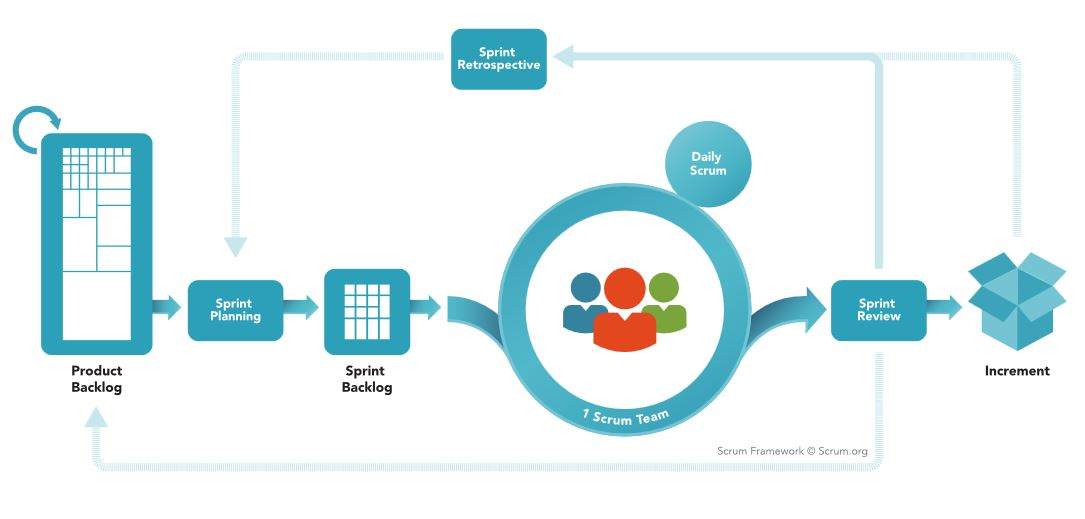
\includegraphics[width=\textwidth]{./3/scrum.png}
	\fonte{\cite{ScrumFramework}}
\end{figure}

\begin{description}
	\item[Product Backlog] funcionalidades ordenadas de acordo com sua import�ncia.
	\item[Sprint Planning] reuni�o para definir o Sprint Backlog.
	\item[Sprint Backlog] lista de funcionalidades a serem implementadas no Sprint.
	\item[Sprint] fase de implementa��o do que foi definido no Sprint Backlog.
	\item[Daily Scrum] reuni�es di�rias para deixar o time a par do desenvolvimento, realizadas via Discord.
	\item[Sprint Review] reuni�o para definir .
	\item[Sprint Retrospective] reuni�o de retrospectiva do Sprint, para definir o que pode ser melhorado no processo.
\end{description}

\section{Cronograma Previsto}

% Definir o cronograma de desenvolvimento do projeto. Elaborar o cronograma por semana, definindo o respons�vel por cada tarefa. O cronograma deve contemplar todas as tarefas previstas no processo de desenvolvimento de software definido para o desenvolvimento do sistema.